\documentclass[12pt, titlepage]{article}

\usepackage{booktabs}
\usepackage{tabularx}
\usepackage{graphicx}
\usepackage{siunitx}
\usepackage{hyperref}
\hypersetup{
    colorlinks,
    citecolor=black,
    filecolor=black,
    linkcolor=red,
    urlcolor=blue
}
\usepackage[round]{natbib}
\usepackage{xr}

%% Comments

\usepackage{color}

\newif\ifcomments\commentstrue

\ifcomments
\newcommand{\authornote}[3]{\textcolor{#1}{[#3 ---#2]}}
\newcommand{\todo}[1]{\textcolor{red}{[TODO: #1]}}
\else
\newcommand{\authornote}[3]{}
\newcommand{\todo}[1]{}
\fi

\newcommand{\wss}[1]{\authornote{blue}{SS}{#1}}
\newcommand{\an}[1]{\authornote{magenta}{Author}{#1}}


%% Common Parts

\newcommand{\progname}{SSP} % PUT YOUR PROGRAM NAME HERE %Every program
                                % should have a name


\externaldocument[SRS-]{../SRS/SRS}
\newcommand{\rref}[1]{R\ref{#1}}
\newcommand{\nfrref}[1]{NFR\ref{#1}}

\externaldocument[MG-]{../Design/MG/MG}
\newcommand{\mref}[1]{M\ref{#1}}

\externaldocument[SVnV-]{../VnVPlan/SystVnVPlan/SystVnVPlan}
\newcommand{\tcref}[1]{TC\ref{#1}}

\externaldocument[UVnV-]{../VnVPlan/UnitVnVPlan/UnitVnVPlan}
\newcommand{\utcref}[1]{TC\ref{#1}}

\begin{document}

\title{Test Report: Slope Stability analysis Program (\progname)} 
\author{Brooks MacLachlan}
\date{\today}
	
\maketitle

\pagenumbering{roman}

\section{Revision History}

\begin{tabularx}{\textwidth}{p{3cm}p{2cm}X}
\toprule {\bf Date} & {\bf Version} & {\bf Notes}\\
\midrule
12/09/18 & 1.0 & First draft of document\\
\bottomrule
\end{tabularx}

~\newpage

\section{Symbols, Abbreviations and Acronyms}

The symbols, abbreviations, and acronyms used in this document include those 
defined in the table below, as well as any defined in the tables found in 
Section~\ref{SRS-sec_RefMat} of the Software Requirements Specification (SRS) 
document.
\newline

\renewcommand{\arraystretch}{1.2}
\begin{tabular}{l l} 
	\toprule		
	\textbf{symbol} & \textbf{description}\\
	\midrule
	MIS & Module Interface Specification\\
	MG & Module Guide\\
	TC & Test Case\\
	VnV & Verification and Validation\\
	\bottomrule
\end{tabular}\\

\newpage

\tableofcontents

\listoftables %if appropriate

\listoffigures %if appropriate

\newpage

\pagenumbering{arabic}

This document outlines the results of testing for \progname{}. 
Section~\ref{sec_FuncReqEval} reports on the tests for functional requirements 
and Section~\ref{sec_NonFuncReqEval} reports on the tests for non-functional 
requirements, all of which are described in the System Verification and 
Validation (VnV) Plan for this project. Section~\ref{sec_Comparison} compares 
this implementation of \progname to the original implementation. 
Section~\ref{sec_UnitTests} reports on the results of the unit tests, which are 
described in the Unit VnV Plan for this project. Section~\ref{sec_Changes} 
comments on changes to the project that that came as a result of the testing. 
Section~\ref{sec_AutoTests} describes how the tests were implemented with an 
automated testing framework. Sections~\ref{sec_TraceReq} and \ref{sec_TraceMod} 
show the traceability between test cases and requirements and modules. 
Supporting documents and other resources, such as the VnVPlans and original 
implementation, can be found on 
\href{https://github.com/smiths/caseStudies/tree/master/CaseStudies/ssp}{the 
GitHub repository for this project}.

\section{Functional Requirements Evaluation} \label{sec_FuncReqEval}

The System VnV Plan described \tcref{SVnV-TC_InvalidSlopeNonMonotonic} - 
\tcref{SVnV-TC_InvalidUnitWtWaterNegative} for testing the requirement for 
verifying that inputs meet physical constraints. All of these tests passed. 

~\newline \noindent The next test in the System VnV Plan, \tcref{SVnV-TC_Ex1FS} 
verified 
the calculation of the factor of safety by comparing it to literature sources 
for a common example problem. The factor of safety calculated by \progname for 
this example problem was 1.3200. The average relative errors between \progname 
and each literature source are shown in Table~\ref{Table:LitFS}. The factor of 
safety calculated by \progname was within 1 percent of all but one of the 
literature sources. The relative tolerance was retroactively set as 0.1 for 
these tests to pass. Note that this test originally failed due to a bug for the 
case where there was no water table, which is discussed further in 
Section~\ref{sec_Changes}.

\begin{table}[!h]
\begin{tabularx}{1.0\textwidth}{p{7cm} l l}
	\toprule \textbf{Source} & \textbf{Factor of Safety} & \textbf{Relative 
	Error}\\ \midrule
	\cite{Greco1996} & 1.3270 & 0.0086\\
	\cite{MalkawiEtAl} & 1.2380 & 0.063\\
	\cite{ChengEtAl} & 1.3250 & 0.0071\\
	\cite{LiEtAl} & 1.3270 & 0.0086\\
	\bottomrule
\end{tabularx}
\caption{Relative error between \progname and literature for calculation of 
factor of safety}
\label{Table:LitFS}
\end{table}

~\newline \noindent The next test in the System VnV Plan, 
\tcref{SVnV-TC_Ex1Slip} 
verified the determination of the critical slip surface again by comparing it 
to literature sources. The average relative errors between \progname and each 
literature source are shown in Table~\ref{Table:LitSlip}. The critical slip 
surface calculated by \progname was within 2 percent of all but one of the 
literature sources. The relative tolerance was retroactively set as 0.1 for 
these tests to pass.

\begin{table}[!h]
\begin{tabularx}{1.0\textwidth}{l p{3.5cm}}
	\toprule \textbf{Source} & \textbf{Relative Error}\\ \midrule
	\cite{Greco1996} & 0.013\\
	\cite{MalkawiEtAl} & 0.072\\
	\cite{ChengEtAl} & 0.013\\
	\cite{LiEtAl} & 0.013\\
	\bottomrule
\end{tabularx}
\caption{Relative error between \progname and literature for calculation of 
critical slip surface}
\label{Table:LitSlip}
\end{table}

~\newline \noindent The next test in the System VnV Plan, 
\tcref{SVnV-TC_OrigProgFS} 
verified the calculation of the factor of safety by comparing it to the 
original implementation for a specific example. The factor of safety calculated 
by \progname for this example problem was 0.9808, compared to 0.9835 for the 
original program. The average relative error between \progname and the original 
program was 0.0027. The relative tolerance was retroactively set as 0.01 for 
these tests to pass.

~\newline \noindent The next test in the System VnV Plan, 
\tcref{SVnV-TC_OrigProgSlip} 
verified the calculation of the critical slip surface by comparing it to the 
original implementation for a specific example. The critical slip surface 
calculated by \progname for this example problem is shown in 
Figure~\ref{Fig:Slip}. The average relative error between \progname and the 
original program was 0.019 The relative tolerance was retroactively set as 0.05 
for these tests to pass.

\begin{figure}[h!]
	\begin{center}
		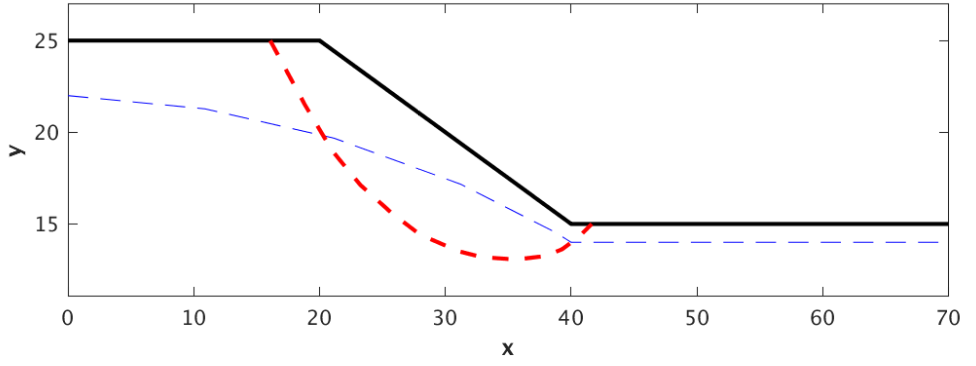
\includegraphics[width=1.0\textwidth]{Slip.png}
		\caption{The critical slip surface for \tcref{SVnV-TC_OrigProgSlip} 
			calculated by \progname{}}
		\label{Fig:Slip}
	\end{center}
\end{figure}

~\newline \noindent The next tests in the System VnV Plan, 
\tcref{SVnV-TC_OrigProgNormal} 
and \tcref{SVnV-TC_OrigProgShear} verified the calculation of the interslice 
normal and shear forces by comparing them the original implementation for a 
specific example. Originally, the relative error between the current 
implementation and the original implementation was unexpectedly high, which led 
to the discovery of a bug in the current implementation, which was then fixed. 
This is discussed further in Section~\ref{sec_Changes}. After fixing the bug, 
the test was performed again. The interslice forces calculated by \progname for 
this example problem are shown in Figure~\ref{Fig:Forces}. The average relative 
error between \progname and the original program was 0.099 for the normal 
forces and 0.072 for the shear forces. These relative errors were still higher 
than expected, but further investigation found that there is a high variance in 
these calculations, even in the original program. For example, the peak 
interslice normal force was seen to vary between about 140 \si{\kilo\newton} 
and 200 \si{\kilo\newton} for different runs of the original program. As a 
result, the tests were given a relatively high relative tolerance of 0.15 and 
were compared to outputs from multiple runs of the original program. As long as 
the relative error is less than the relative tolerance for at least one of the 
outputs, the tests pass. With these changes, both tests pass on the vast 
majority of runs.

\begin{figure}[h!]
	\begin{center}
		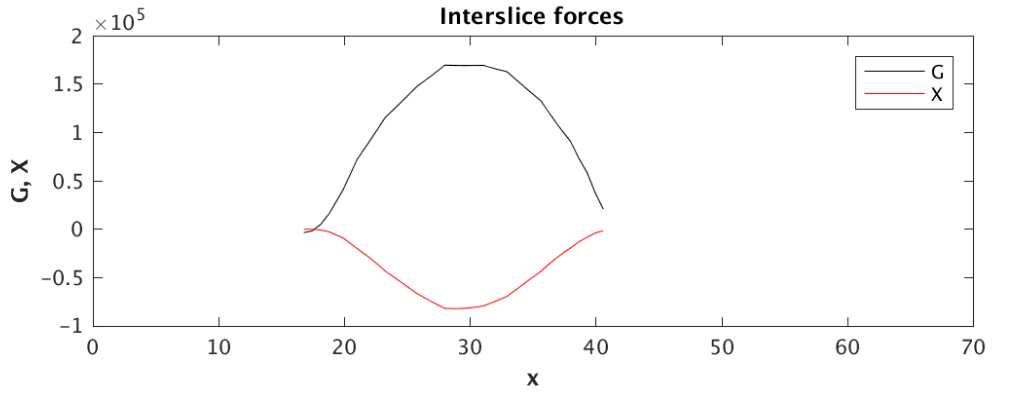
\includegraphics[width=1.0\textwidth]{Forces.png}
		\caption{The interslice normal and shear forces for  
		\tcref{SVnV-TC_OrigProgNormal} and  \tcref{SVnV-TC_OrigProgShear}
			calculated by \progname{}}
		\label{Fig:Forces}
	\end{center}
\end{figure}

~\newline \noindent The next test in the System VnV Plan, 
\tcref{SVnV-TC_CalcConstantf}, 
verified that changing the type of the function $f$ to a constant has an impact 
on the result. This was done by visual inspection of the critical slip surface 
and interslice forces for the case where \textit{const\_f} is true. These plots 
are shown in Figure~\ref{Fig:ConstF}. The factor of safety was 0.8363 for this 
test. The results were similar overall to the case where \textit{const\_f} was 
false, with some notable differences: A slightly higher exit x-value for the 
slip surface, associated with notably different interslice forces near the 
exit, and an approximately 14 percent difference in factor of safety. These 
slight differences give confidence that \progname actually translated the 
\textit{const\_f} input to a different $f$ function, which is what this test 
was checking for, and thus the test was considered a pass.

\begin{figure}[h!]
	\begin{center}
		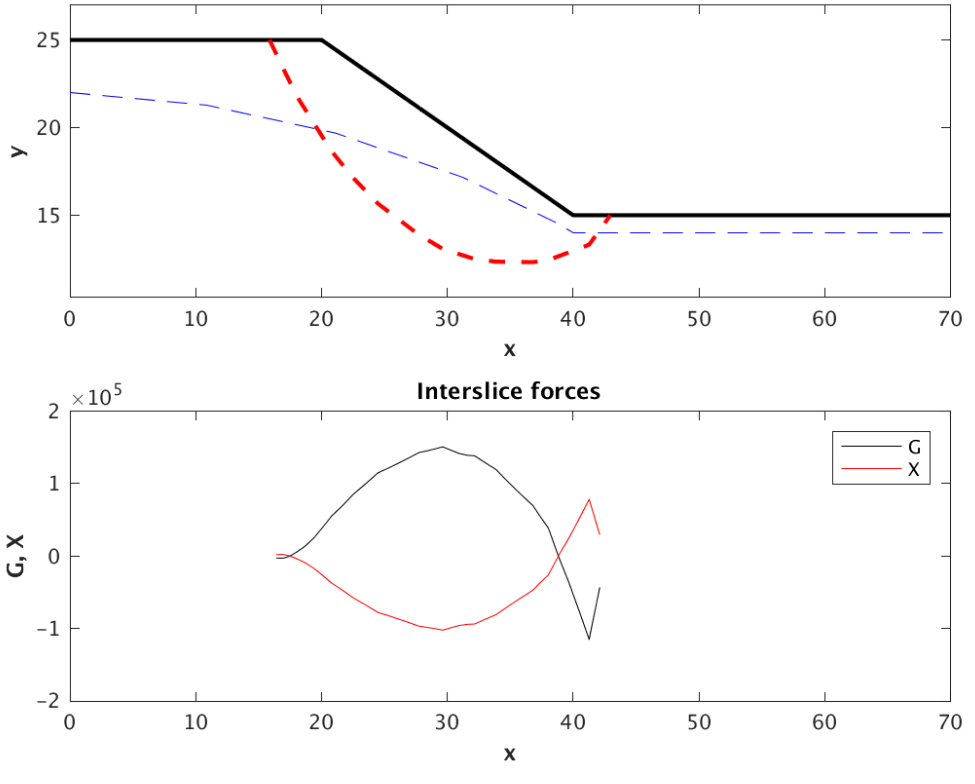
\includegraphics[width=1.0\textwidth]{ConstFPlots.png}
		\caption{The critical slip surface (top) and interslice normal and 
		shear forces (bottom) for  \tcref{SVnV-TC_CalcConstantF} calculated by 
		\progname{}}
		\label{Fig:ConstF}
	\end{center}
\end{figure}

~\newline \noindent The final tests in the System VnV Plan, 
\tcref{SVnV-TC_OutputInputXEtrMin} - \tcref{SVnV-TC_ValidOutFS}, were for 
verifying the requirements for verifying and delivering output. These tests all 
passed.

\section{Nonfunctional Requirements Evaluation} \label{sec_NonFuncReqEval}

\subsection{Maintainability}
		
\subsection{Reusability}
	
\section{Comparison to Existing Implementation} \label{sec_Comparison}

This section will not be appropriate for every project.

\section{Unit Testing}  \label{sec_UnitTests}

\section{Changes Due to Testing} \label{sec_Changes}
- bug with NoWT and constraint (found by system test)
- bug with mirrored forces (found by last system test)
- bug with indivisible slices (found by slice tests)

\section{Automated Testing} \label{sec_AutoTests}
		
\section{Trace to Requirements} \label{sec_TraceReq}
		
\section{Trace to Modules} \label{sec_TraceMod}

\section{Code Coverage Metrics}
Not applicable for \progname.

\bibliographystyle{plainnat}

\bibliography{../../refs/References}

\end{document}